\documentclass[12pt,letter]{article}
\usepackage{../downey_format}




\begin{document}
	
%	\large{}
%	
%	\title{\vspace{-2cm} Chapter 5: Basic concepts of Control Theory}
%	\date{}
%	\maketitle

	% set the section number, along with figure and equation numbers
	\setcounter{section}{9}	
	\setcounter{figure}{\thesection}   
	\renewcommand\thefigure{\thesection.\arabic{figure}}
	\setcounter{equation}{\thesection}   
	\renewcommand\theequation{\thesection.\arabic{equation}}

\section{Control Systems Designer}

The Control System Designer is a MATLAB SISO Tool.

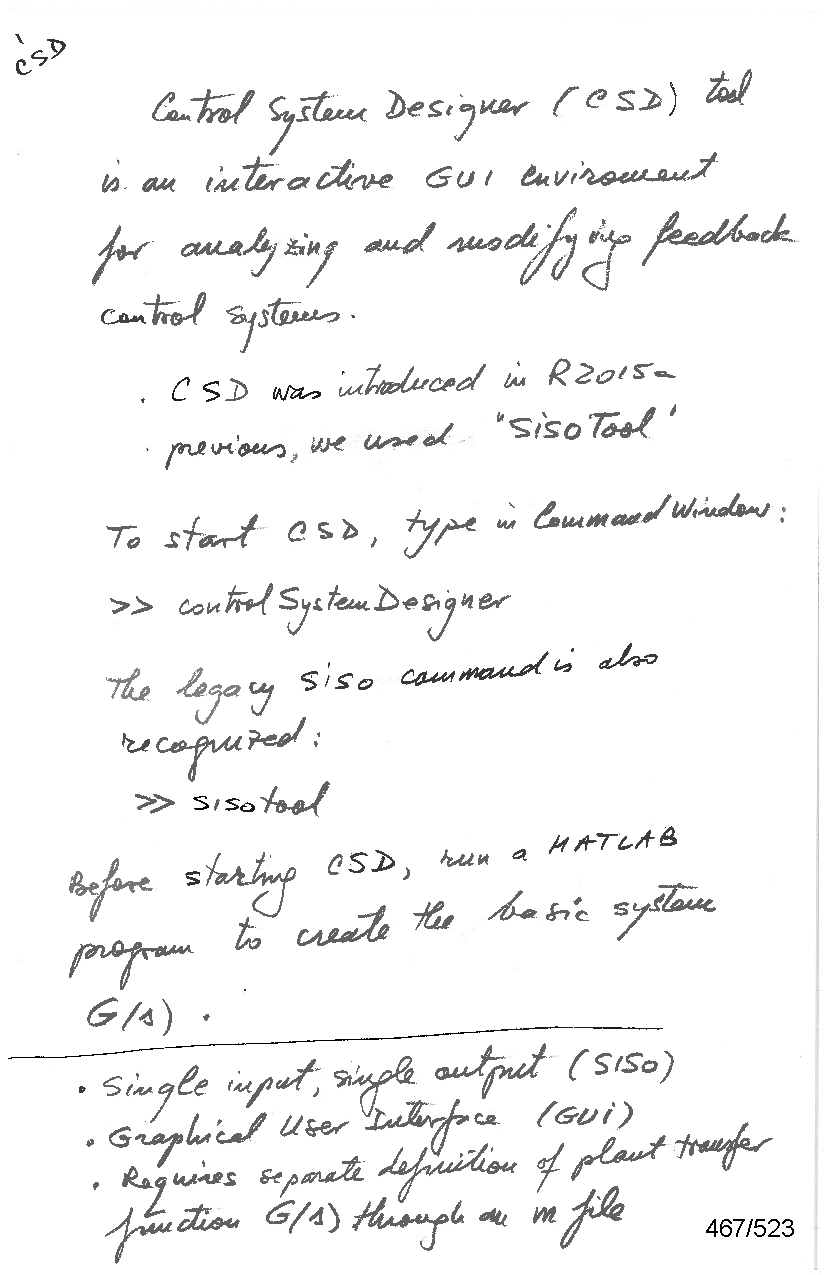
\includepdf[pages=-,pagecommand={},width=0.9\textwidth]{PDF_notes/Control_Systems_Designer.pdf}









	\pagebreak
	\renewcommand{\thepage}{}
	\renewcommand\refname{References Cited}
	\pagestyle{plain}
	\bibliographystyle{Downey_NSF}
	\bibliography{Chapter_1_Basic_Concepts}


















\end{document}

